\documentclass[
  11pt,
  letterpaper,
   addpoints,
   answers
  ]{exam}

\usepackage{../exercise-preamble}

\begin{document}

\noindent
\begin{minipage}{0.47\textwidth}

\includegraphics[width=\textwidth]{../fcfm_die}
\end{minipage}
\begin{minipage}{0.53\textwidth}
\begin{center} 
\large\textbf{Conversión de la Energía y Sistemas Eléctricos } (EL4111-1) \\
\large\textbf{Clase auxiliar 3} \\
\small Prof.~Constanza Ahumada - Rodrigo Moreno.\\
\small Prof.~Aux.~Javiera Pacheco - Erik Sáez\\
\small Ayudantes.~Manuel Aceituno - Pamela Acuña - Alvaro Flores\\
\end{center}
\end{minipage}

\vspace{0.5cm}
\noindent
\vspace{.85cm}

\begin{questions}
    %%%%%%%%%%%%%%%%%%%%%%%%%%%
    \question Considere el siguiente circuito electromecánico, el cual presenta permeabilidad infinita en el material ferromagnético, y cada devanado posee un número de vueltas \( N_1 = N_2 = 200 \, [\text{vueltas}] \), los cuales están conectados en serie. Además, los entrehierros del circuito son todos iguales, de longitud variable \( x \) y área \( A = 4 \, [\text{cm}^2] \). Por último, en la parte inferior del núcleo cuelga un péndulo cuya masa es igual a \( M = 3 \, [\text{kg}] \), y ambos se encuentran levantados debido a la acción del campo magnético y de un resorte, cuya constante elástica es \( K = 10.000 \, [\text{kg/s}^2] \) y su largo natural es de \( x_0 = 5 \, [\text{mm}] \).
    \begin{figure}[h!]
        \centering
        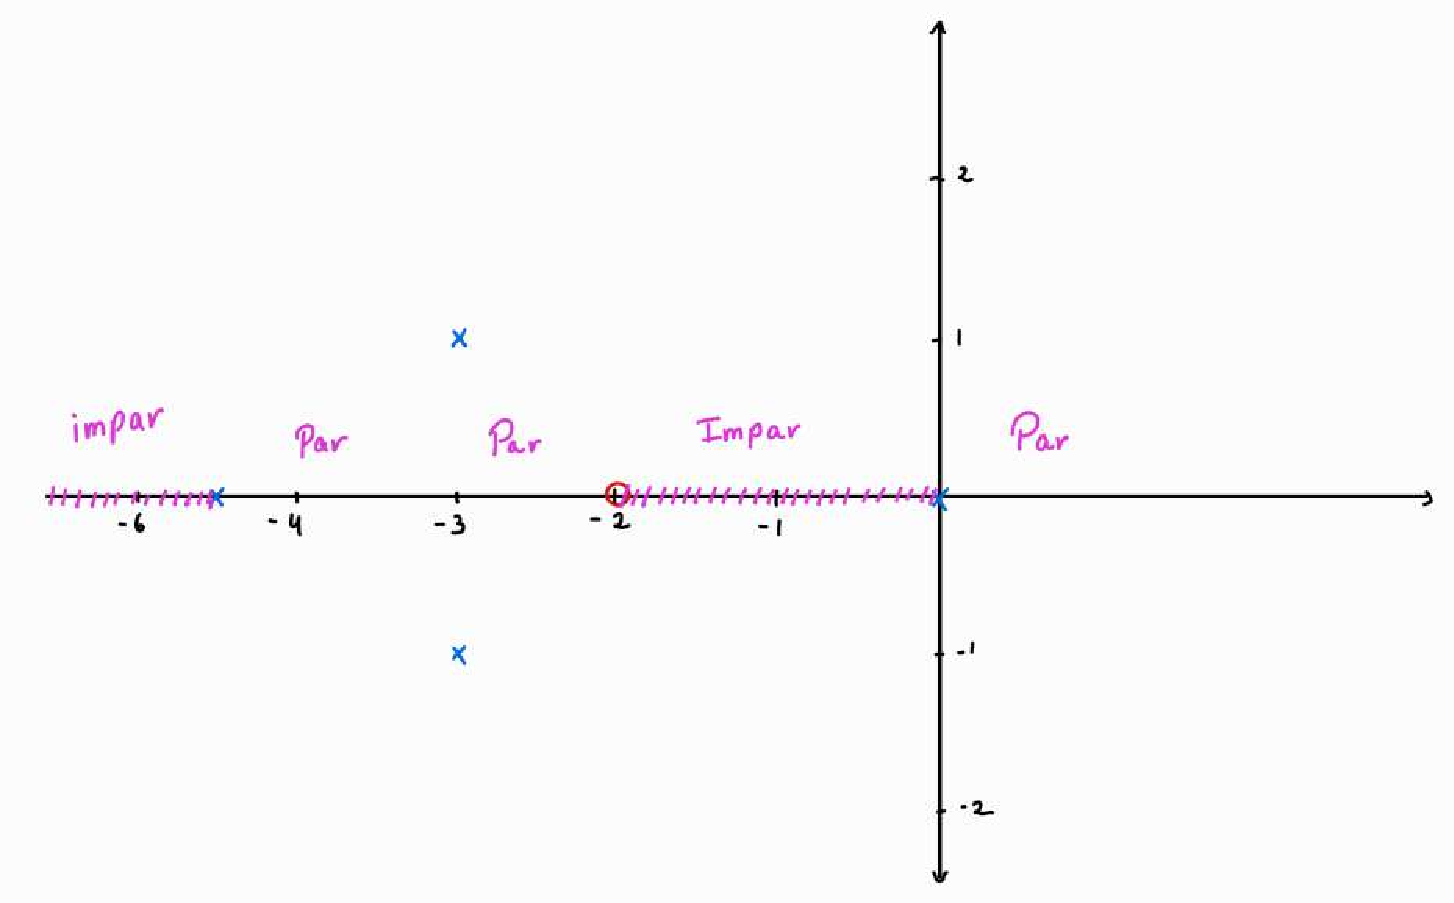
\includegraphics[width=0.45\textwidth]{Auxiliar_2_1}
        \caption{Circuito electromecánico.}
    \end{figure}

    \begin{enumerate}
        \item[(a)] Determinar la reluctancia de cada entrehierro y las inductancias propias y mutuas del circuito magnético en función de la corriente \( i \) y de la longitud \( x \) del entrehierro.
        \item[(b)] Determinar la energía y la fuerza magnética.
        \item[(c)] Escribir la ecuación dinámica que modela el sistema electromecánico, escogiendo de manera adecuada el sistema de referencia a utilizar.
        \item[(d)] Determinar la corriente por las bobinas, en estado estacionario, para las siguientes longitudes del entrehierro:
        \begin{itemize}
            \item \( 5 \, [\text{mm}] \)
            \item \( 6 \, [\text{mm}] \)
            \item \( 4 \, [\text{mm}] \)
        \end{itemize}
    \end{enumerate}
    %%%%%%%%%%%%%%%%%%%%%%%%%%%
    \begin{solution}
        \subsection*{Resolución 1.1}
        Se pide determinar reluctancia entre los entre hierros,inductancias propias y mutuas en funcion de la corriente y la longitud del entre hierra, por lo tanto para el primer primer caso tenemos que todos los entre hierros son iguales, por lo que se tiene que la reluctancia vendra dada por:
        \begin{align}
            R(x) = \frac{x}{\mu_{0}A}
        \end{align}
        Que es en funcion del entrehierro, ademas se desprecia la reluctancias de los nucleos dado que $\mu \rightarrow \infty$. Para las inductancias mutuas se tendra que plantear el circuito magnetico , el cual viene dado por:
        \begin{center}
            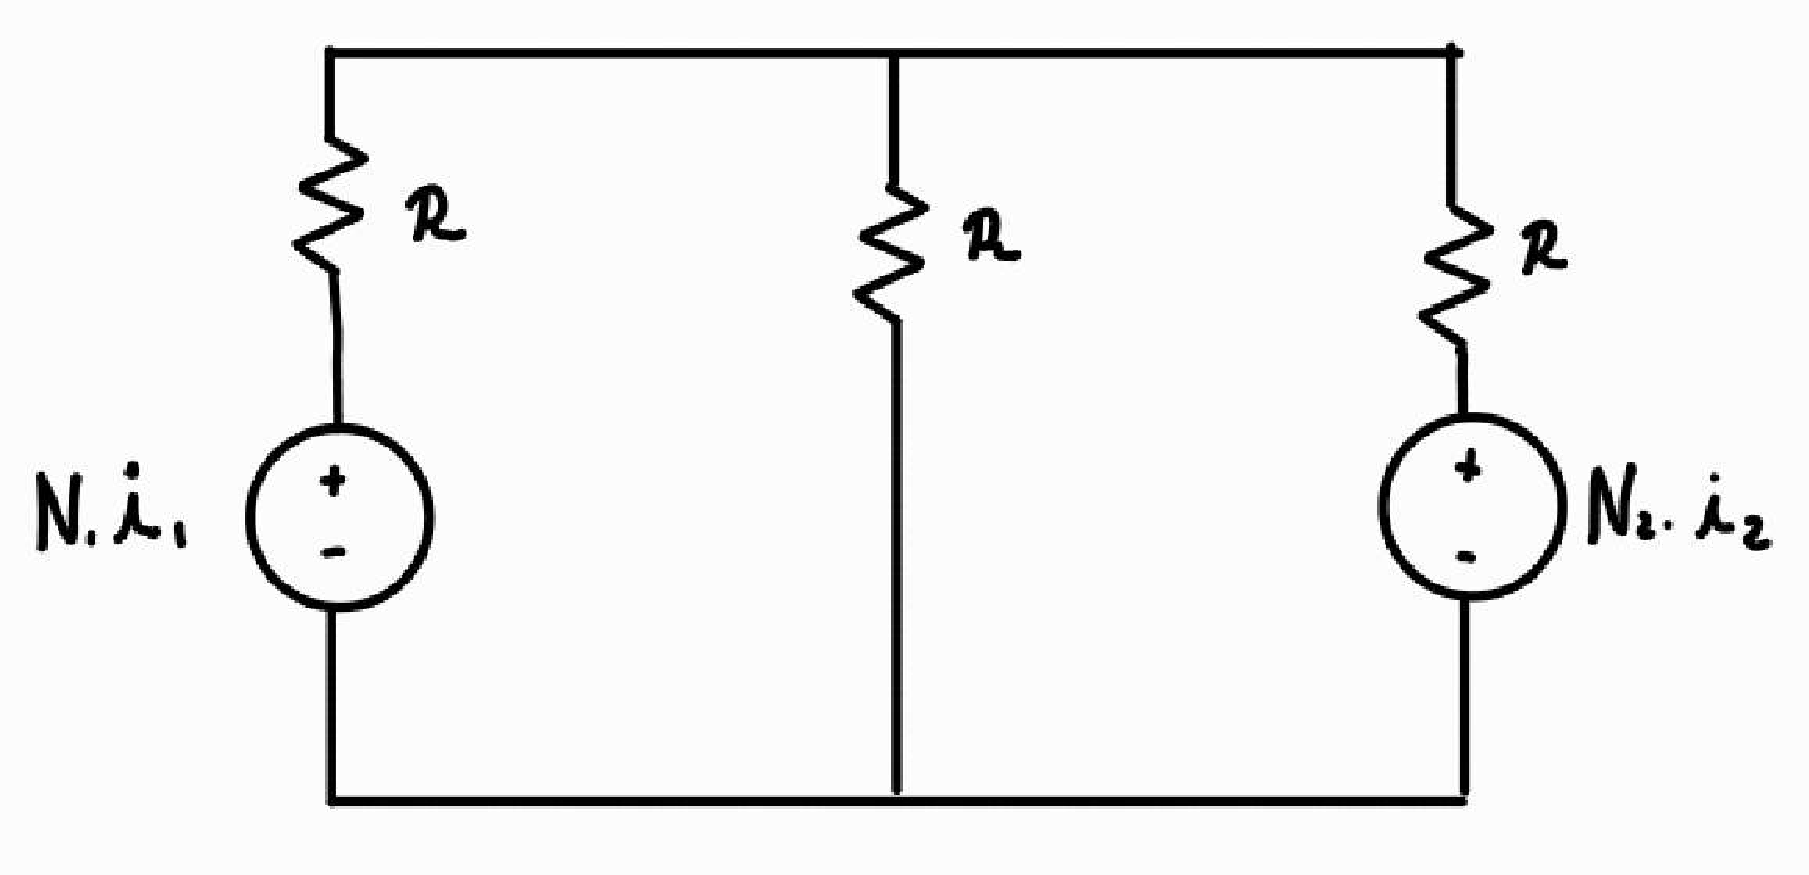
\includegraphics[width=0.4\textwidth]{Auxiliar_2_2}
        \end{center}
        Recordamemos que la inductancia se asocia de manera directa con los flujos magneticos involucrados, por lo tanto si se desea obtener $L_{11}$ esta vendra asociada unicamente a el flujo asociada a la fuente magnetomotriz que lo genera, por lo que podemos omitir el resto (\textit{Equivalentemente a apagar las fuentes}), dado que no nos interesa el efecto de estas sobre la bobina que queremos obtener (\textit{Inductancia mutua}), por lo tanto tenemos el siguiente esquema:
        \begin{center}
            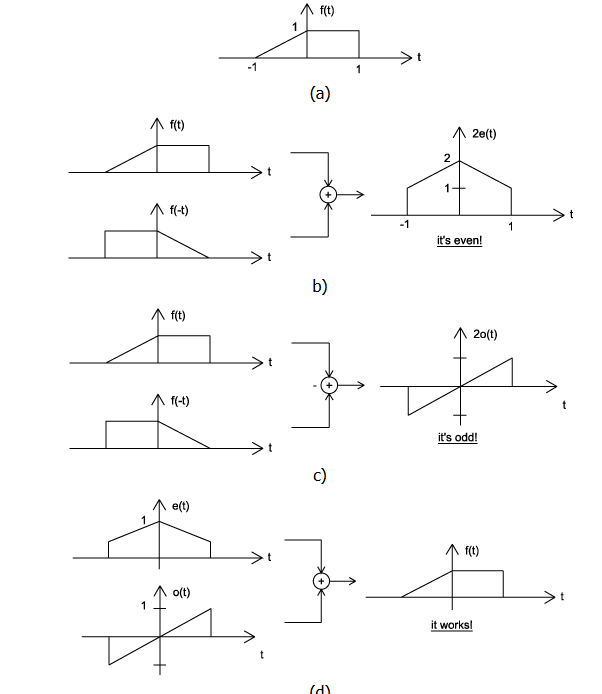
\includegraphics[width=0.4\textwidth]{Auxiliar_2_3}
        \end{center}
        Luego tendremos por tanto que:
        \begin{align}
            N_{1}I_{1}= \phi_{11}R_{eq}
        \end{align}
        Dado que la corriente que genera ambas fuentes magnetomotriz asi como su numero de vueltas es el mismo, por lo que se tiene que:
        \begin{align}
            N \cdot I = \phi_{11} \cdot R_{eq}
        \end{align}
        De esta manera en base al circuito magnetomotriz visto en la imagen anterior tenemos que:
        \begin{align}
            N \cdot I &= \phi_{11} \cdot (R// + R)\\
            N \cdot I &= \phi_{11} \cdot \frac{3}{2}R\\
            \phi_{11} &= \frac{2N \cdot I}{3R}
        \end{align}
        Que si reemplazamos el valor de la reluctancia se tendra:
        \begin{align}
            \phi_{11} &= \frac{2N \cdot I}{\left(3\frac{x}{\mu_{0}A}\right)}\\
            \phi_{11} &= \frac{2N \cdot I \mu_{0}A}{3x}
        \end{align}
        Por lo que finalmente la inductancia propia $L_{11}$ vendra dada por:
        \begin{align}
            L_{11} = \frac{\phi_{11}}{I} = \frac{2N^{2} \mu_{0}A}{3x}
        \end{align}
        Para obtener $L_{22}$ notamos que el sistema es equivalente con lo que se tiene que:
        \begin{align}
            L_{22} = \frac{2N^{2} \mu_{0}A}{3x}
        \end{align}
        Luego se busca el obtener la inductancia mutua $L_{21}$, por lo que ahora se considera el efecto de la segunda bobina sobre la primera, que en terminos del circuito magnetico , equivale a apagar la segunda fuente pero considerar el flujo que esta genera, por lo que se tiene el siguiente esquema:
        \begin{center}
            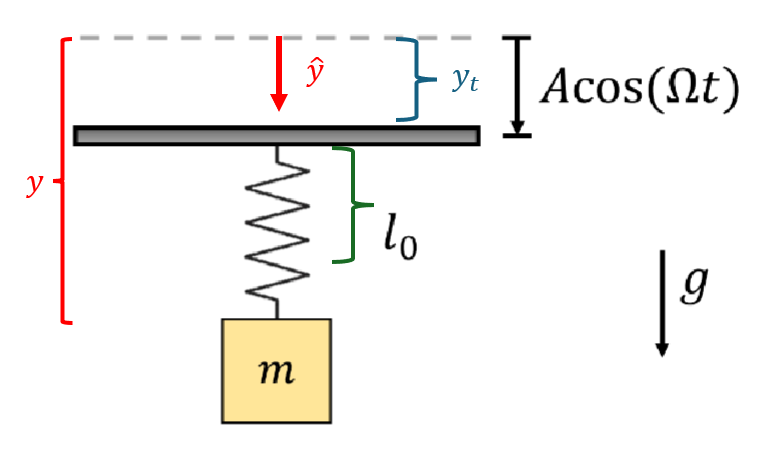
\includegraphics[width=0.4\textwidth]{Auxiliar_2_4}
        \end{center}
        Luego este se puede resolver por el metodo  que consideren apropiado, es directo ver que se puede resolver por division de corriente. En este caso particular tomare una mala en la zona derecha del circuito, con lo que se tiene que:
        \begin{align}
            R(\phi_{21} + \phi_{11})+ R\phi_{21}= 0\\
            \phi_{21} = -\frac{\phi_{11}}{2}
        \end{align}
        que reemplazando se obtiene que:
        \begin{align}
            \phi_{21} = -\frac{N \cdot I \mu_{0}A}{3x}
        \end{align}
        Con lo que su inductancia mutua vendra dado por:
        \begin{align}
            L_{21} = \frac{\phi_{21}}{I} = -\frac{N^{2} \mu_{0}A}{3x}
        \end{align}
        Para el caso de $L_{12}$ se tiene que el circuito es simetrico con lo que:
        \begin{align}
            L_{12} = -\frac{N^{2} \mu_{0}A}{3x}
        \end{align}
        Finalmente se obtiene lo pedido.
        \subsection*{Resolucion 1.2}
        Se busca el obtener la energia magnetica y la fuerza magnetica. Para obtener la primera $W_{field}$ se tiene que:
        \begin{align}
            \Delta W &= \int_{t_{1}}^{t_{2}} p \, dt = \int_{\lambda_{1}}^{\lambda_{2}} i \, d\lambda = \int_{\lambda_{1}}^{\lambda_{2}} \frac{d\lambda}{dt} \, dt = \int_{\lambda_{1}}^{\lambda_{2}} \frac{\lambda}{L} \, d\lambda \\
            &= \frac{1}{2L} \left( \lambda_{2}^{2} - \lambda_{1}^{2} \right)
            \end{align}
        Donde se considera que $\lambda_{1}= 0$ es decir que $W_{field} = \frac{1}{2}Li^{2}$ que es equivalente a decir que consideramos la energia magnetica de cada fuente de manera independiente. Por lo que generelizando para el caso de dos bobinas tendremos que:
        \begin{align}
            W_{field} = \frac{1}{2}L_{11}i_{1}^{2} + \frac{1}{2}L_{22}i_{2}^{2} + L_{12}i_{1}i_{2} + L_{21}i_{1}i_{2}
        \end{align}
        Reemplazando sobre las inductancias obtenidas con anterioridad, se tiene que (\textit{Notar que todas las corrientes son iguales, al igual que las indutralcias propias y mutuas}):
        \begin{align}
            W_{field}&= Li^{2} + Mi^{2}\\
                     &= \frac{2N^{2}\mu_{0}Ai^{2}}{3x} - \frac{N^{2}\mu_{0}Ai^{2}}{3x}\\
                        &= \frac{N^{2}\mu_{0}Ai^{2}}{3x} 
        \end{align} 
        De esta manera se obtiene la energia magnetica. Por otro lado para obtener la fuerza magnetica se tiene que:
        \begin{align}
            F_{m} = \frac{-dW_{field}}{dx} = \frac{N^{2}\mu_{0}Ai^{2}}{3x^{2}}
        \end{align}
        Con lo que se obtiene la fuerza magnetica.
        \subsection*{Resolucion 1.3}
        Se busca obtener la ecuacion dinamica del sistema, para esto se tiene que considerar el sistema de referencia adecuado, por lo que se tiene que considerar el sistema de referencia que se muestra en la imagen, con lo que se tiene que:
        \begin{center}
            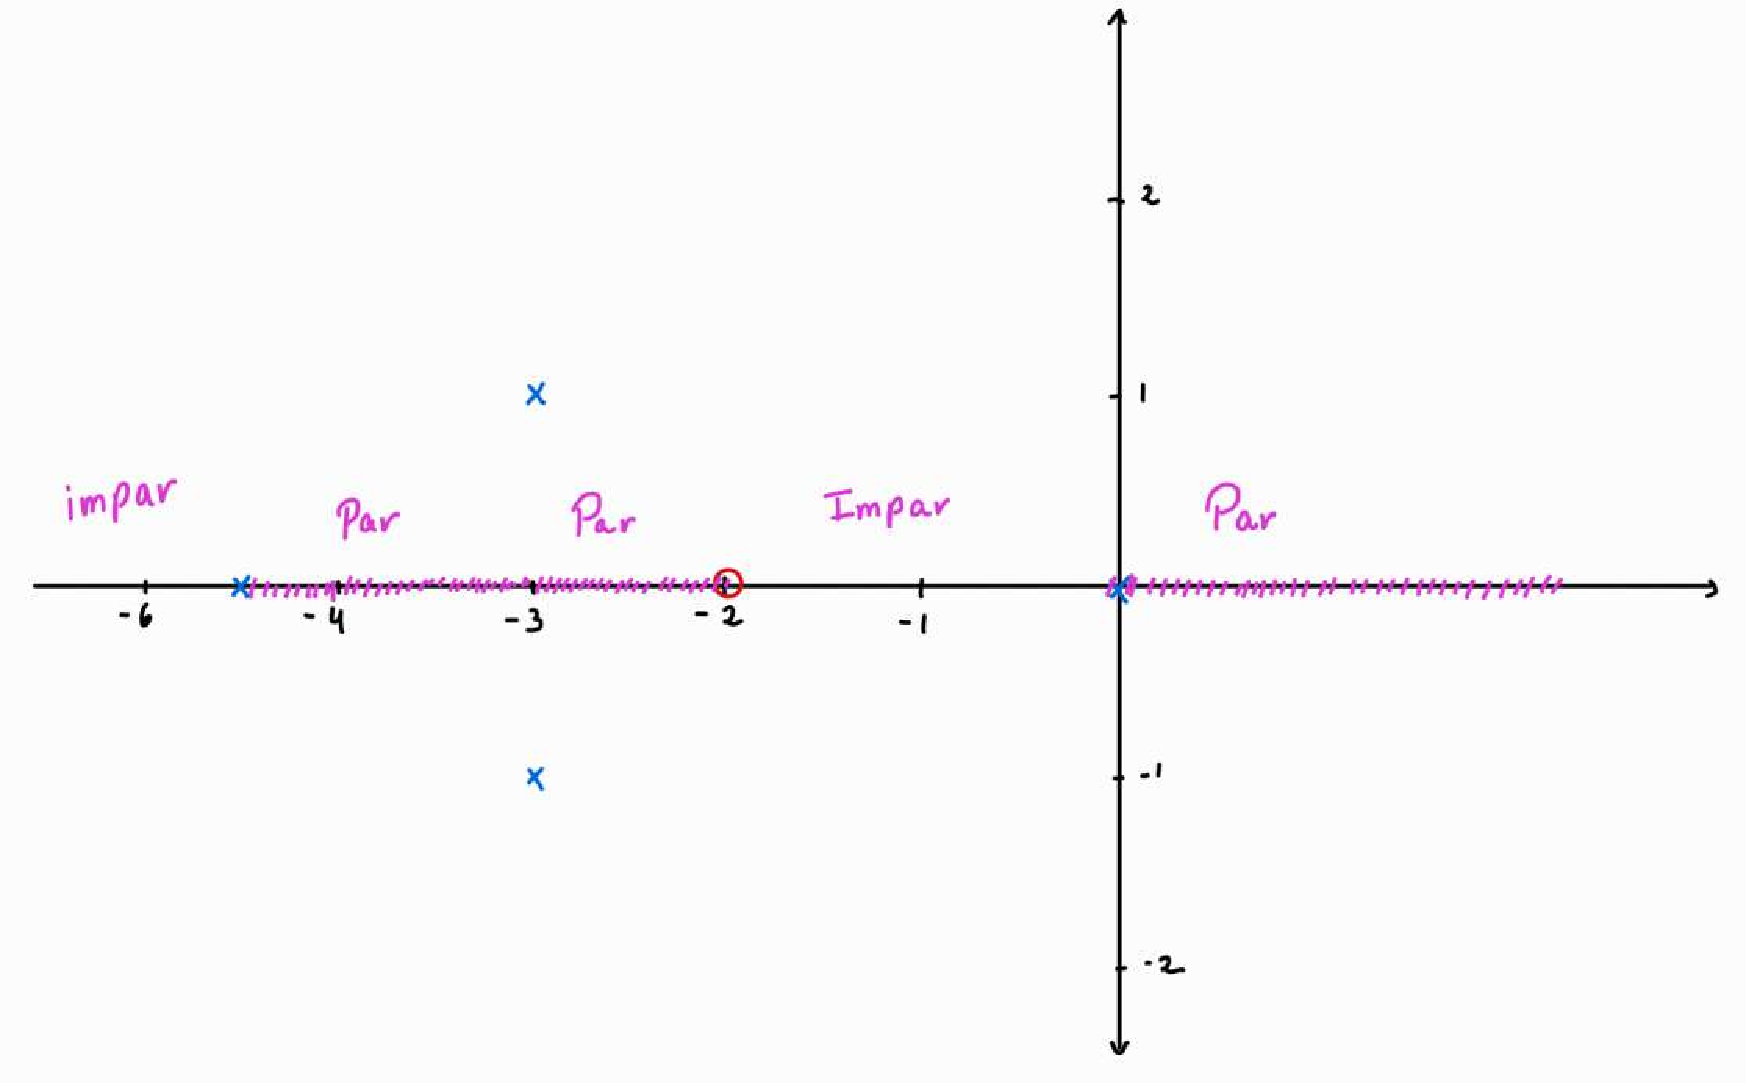
\includegraphics[width=0.4\textwidth]{Auxiliar_2_5}
        \end{center}
        Luego tenemos varias fuerzas involucradas en el sistema,por lo tanto aplicando , la segunda ley de Newton se tiene que:
        \begin{align}
            \sum F &= M\ddot{x}\\
            f_{field} + f_{resorte} + f_{peso} &= M\ddot{x}\\
            Mg - k(x-l_{0}) - \frac{N^{2}\mu_{0}Ai^{2}}{3x^{2}} &= M\ddot{x}
        \end{align}
        Con lo que se obtiene el modelo mecanico del sistema visto anteriormente.
        \subsection*{Resolucion 1.4}
        Se busca obtener la corriente por las bobinas y la magnitud de cada fuerza involucrada, en estado estacionario, esto ultimo hace referencia que se debera cumplir que $\ddot{x}= \dot{x}=0$, con lo que volviendo sobre nuestra ecuacion dinamica se tiene que:
        \begin{align}
            Mg - k(x-l_{0}) - \frac{N^{2}\mu_{0}Ai^{2}}{3x^{2}} &= 0 
        \end{align}
        Como nos interesa obtener la corriente, la despejamos del termino anterior tal que:
        \begin{align}
            i = \sqrt{\frac{3x^{2}(Mg - k(x-l_{0}))}{N^{2}\mu_{0}A}}
        \end{align}
        Luego dado que nos interesa el valor numerico de cada componente tenemos que:
        \begin{itemize}
            \item Para $x = 5[mm] = 0.005[m]$
            \begin{align}
                i &= \sqrt{\frac{3 \cdot (0.005)^2}{(200)^2 \cdot 4\pi \cdot 10^{-7} \cdot 0.0004} \cdot \left[3 \cdot 9.8 - 10000 \cdot \left(0.005 - 0.005\right)\right]} \\
                i &= 10.4722 \, \text{[A]}
            \end{align}
            \item Para $x = 6[mm] = 0.006[m]$
            \begin{align}
                i &= \sqrt{\frac{3 \cdot (0.006)^2}{(200)^2 \cdot 4\pi \cdot 10^{-7} \cdot 0.0004} \cdot \left[3 \cdot 9.8 - 10000 \cdot \left(0.006 - 0.005\right)\right]} \\
                i &= 10.2081 \, \text{[A]}
            \end{align}
            \item Para $x = 4[mm] = 0.004[m]$
            \begin{align}
                i &= \sqrt{\frac{3 \cdot (0.004)^2}{(200)^2 \cdot 4\pi \cdot 10^{-7} \cdot 0.0004} \cdot \left[3 \cdot 9.8 - 10000 \cdot \left(0.004 - 0.005\right)\right]} \\
                i &= 9.6984 \, \text{[A]}
            \end{align}
        \end{itemize}
        Con lo que finalmente se obtiene la corriente por las bobinas.
    \end{solution}
    %%%%%%%%%%%%%%%%%%%%%%%%%%%
    \question Sea el siguiente esquema de un funcionamiento electromecanico:
    \begin{center}
        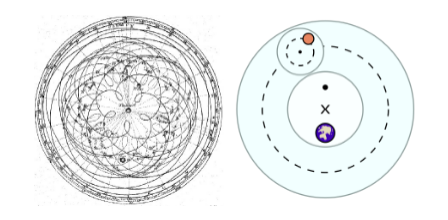
\includegraphics[width=0.65\textwidth]{Auxiliar_2_10}
    \end{center}  
    \begin{enumerate}
        \item Determine las ecuaciones que modelan el sistema mecanico y electrico.
        \item \textbf{Propuesto} Analice la posicion de su sistema cuando la corriente es constante (Conocida $I_{0}$) y el sistema esta en equilibrio. 
    \end{enumerate}
%%%%%%%%%%%%%%%%%%%%%%%%%%%
\begin{solution}
\subsection*{Resolucion 2.1}
   Dado el esquema, se busca obtener las ecuaciones que modelan el sistema mecanico, por lo que se tiene que considerar las fuerzas involucradas en el sistema, en particular nos interesa la fuerza magnetica, por lo que se tiene el siguiente esquema:
   \begin{center}
    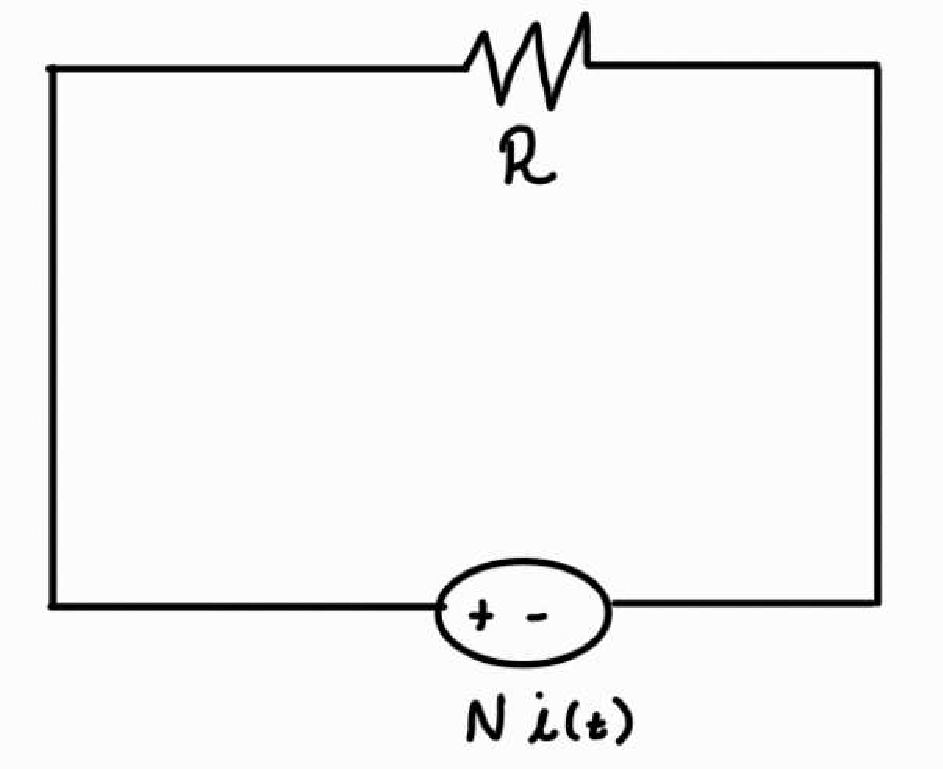
\includegraphics[width=0.3\textwidth]{Auxiliar_2_6}
\end{center}
   Luego tenemos que al tener unicamente una fuente magnetica y despreciando la reluctancia del nucleo, el sistema se reduce a:
   \begin{align}
     Ni(t) = \phi(t)R_{eq}
   \end{align}
   Notamos que la corriente dependera del tiempo. Tenemos por tanto que la reluctancia vendra dada por:
    \begin{align}
      R_{g} = \frac{(l_{1}-x(t))}{A \mu_{0}}
    \end{align}
    Con lo que $\phi(t)$ vendra dado por:
    \begin{align}
        Ni(t) &= \phi(t) \frac{(l_{1}-x(t))}{A \mu_{0}}\\
        \phi(t) &= \frac{Ni(t)A\mu_{0}}{(l_{1}-x(t))}
    \end{align}
    Lo relacionamos con la inductancia tal que:
    \begin{align}
        L(t) &= \frac{\phi(t)N}{i(t)}\\
             &= \frac{A\mu_{0}N^{2}}{(l_{1}-x(t))}
    \end{align}
    De esta manera se logra obtener la energia magnetica la cual viene dada por:
    \begin{align}
        W_{field} &= \frac{1}{2}L(x(t))(i(t))^{2}\\
                 &= \frac{A\mu_{0}N^{2}i^{2}}{2(l_{1}-x(t))}
    \end{align}
    Por lo que la fuerza magnetica correspondera a:
    \begin{align}
        F_{m} &= -\frac{dW_{field}}{dx}\\
              &= \frac{A\mu_{0}N^{2}i^{2}}{2(l_{1}-x(t))^{2}}
    \end{align}
    Con lo que finalmente se obtiene que el ssitema mecanico vendra expresado por:
    \begin{align}
        M\ddot{x} &= f_{m} - f_{e} - M\dot{x}\\
                  &=\frac{A\mu_{0}N^{2}i^{2}}{2(l_{1}-x(t))^{2}} - k(x-l_{0}) - B\dot{x}
    \end{align}
    Por otro lado se busca obtener el modelo electrico el cual viene dado de manera simplicada por:
    \begin{center}
        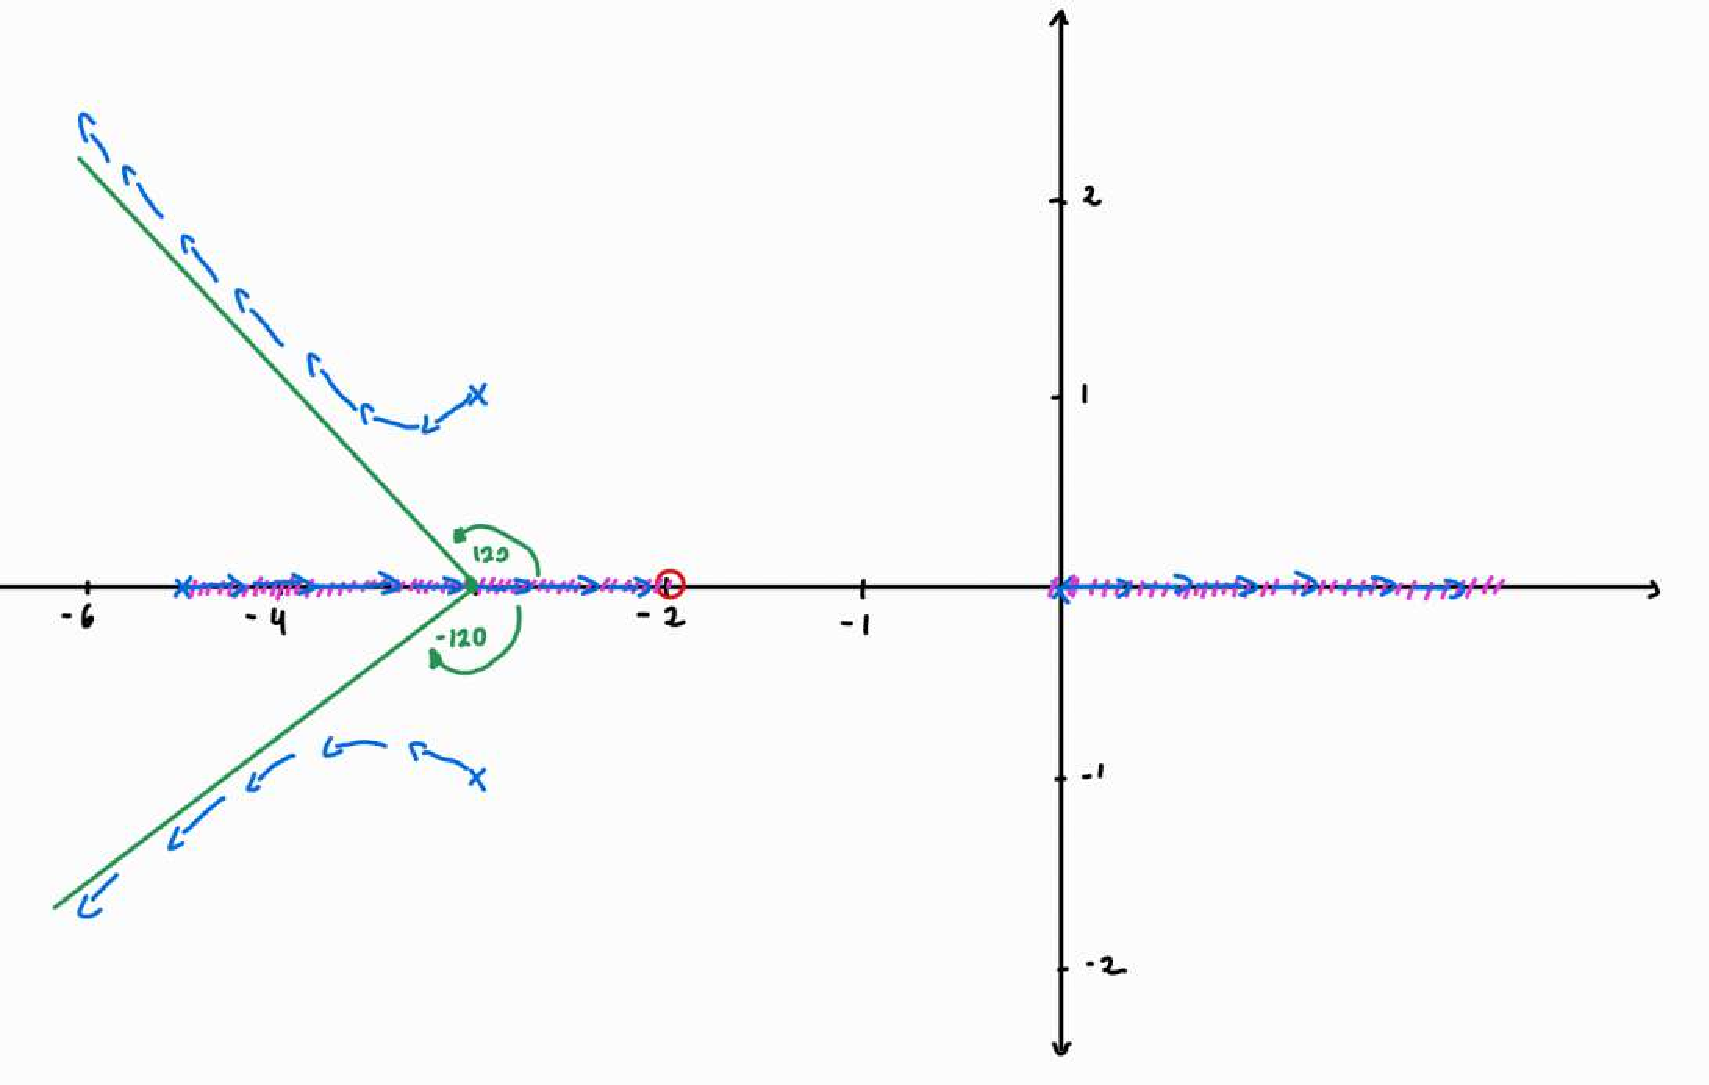
\includegraphics[width=0.4\textwidth]{Auxiliar_2_7}
    \end{center}
    Con lo que mediante una malla simple se obtiene:
    \begin{align}
        \epsilon(t) = Ri(t) + \frac{d L(x(t))i(t)}{dt}
    \end{align}
    Es interesante notar que en esta ocacion la inductancia no sera constante, por lo que no sale directamente de la derivada, asi tenemos que:
    \begin{align}
        \epsilon(t) &= i(t)R + \frac{dL(x(t))}{dt}i(t) + L(x(t))\frac{d i(t)}{dt}
    \end{align}
    Reemplazando se obtiene:
    \begin{align}
        \epsilon(t) &= i(t)R + \frac{A\mu_{0}N^{2}i(t)}{2(l_{1}-x(t))^{2}}\left[\frac{dx}{dt}\right] + \frac{A\mu_{0}N^{2}(t)}{2(l_{1}-x(t))}\left[\frac{di}{dt}\right]
    \end{align}
    Con lo que finalmente se obtienen los dos pares de ecuaciones que modelan el circuito electromecanico:
    \begin{align}
        M\ddot{x} &= \frac{A\mu_{0}N^{2}i^{2}}{2(l_{1}-x(t))^{2}} - k(x-l_{0}) - B\dot{x}\\
        \epsilon(t) &= i(t)R + \frac{A\mu_{0}N^{2}i(t)}{2(l_{1}-x(t))^{2}}\left[\frac{dx}{dt}\right] + \frac{A\mu_{0}N^{2}}{2(l_{1}-x(t))}\left[\frac{di}{dt}\right]
    \end{align}
 \end{solution}
%%%%%%%%%%%%%%%%%%%%%%%%%%%
\question Se tiene el circuito visto en la Figura , el cual se desea analizar considerando los siguientes supuestos:
\begin{itemize}
    \item El conductor que compone cada bobina no tiene resistencia eléctrica.
    \item Todo el flujo generado por la bobina primaria es enlazado por la bobina secundaria, es decir no hay flujos de fuga.
    \item No hay pérdidas por histéresis ni corrientes parásitas.
    \item La permeabilidad del núcleo es muy alta (infinita), por lo que se requiere una fuerza magnetomotriz (relacionada con la corriente de excitación) muy pequeña que es posible ignorar para establecer el flujo.
\end{itemize}
\begin{center}
    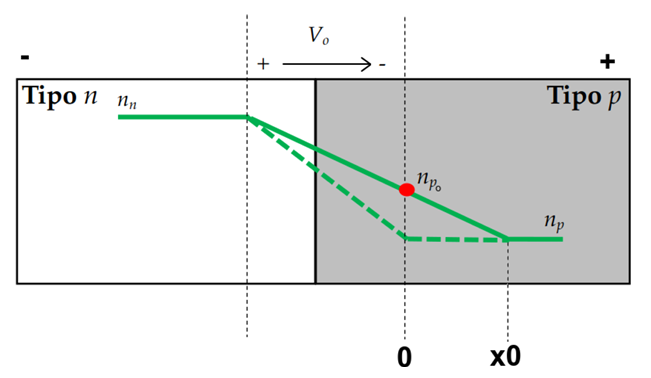
\includegraphics[width=0.65\textwidth]{Auxiliar_2_11}
\end{center}
\begin{enumerate}
    \item Indicar la polaridad de los transformadores, nombrándolas y dibujando los puntos
    correspondientes
    \item Calcular la potencia de ambas cargas \( Z_1 \) y \( Z_2 \), considerando \( V = 110\text{[V]}\angle 0^{\circ} \), \( Z_1 = Z_2 = 20 + j\ \Omega \), \( N_1 = 30 \) y \( N_2 = 60 \).
    \item  Calcular la potencia de la fuente, considerando \( V = 110\text{[V]}\angle 0^\circ \), \( Z_1 = 20 + j[ \Omega] \), \( N_1 = 30 \), \( N_2 = 60 \) y dos casos para \( Z_2 \) con \( Z_2 = 0 \) y \( Z_2 = \infty \).
    \item Determine la energía almacenada en el campo magnético de cada bobina.
\end{enumerate}

%%%%%%%%%%%%%%%%%%%%%%%%%%%
\begin{solution}
    \subsection*{Resolucion 3.1}
    Dado que se busca indicar la polaridad de los transformadores, se debe identificar de manera visual y haciendo uso de la regla de la mano derecha, la polaridad de los transformadores, es por esto que el transformador de la izquierda se observa que su polaridad es \textbf{sustractiva} mientras que la del transformador de la derecha es \textbf{aditiva}, por lo que dibujando los puntos correspondientes se tiene:
    \begin{center}
        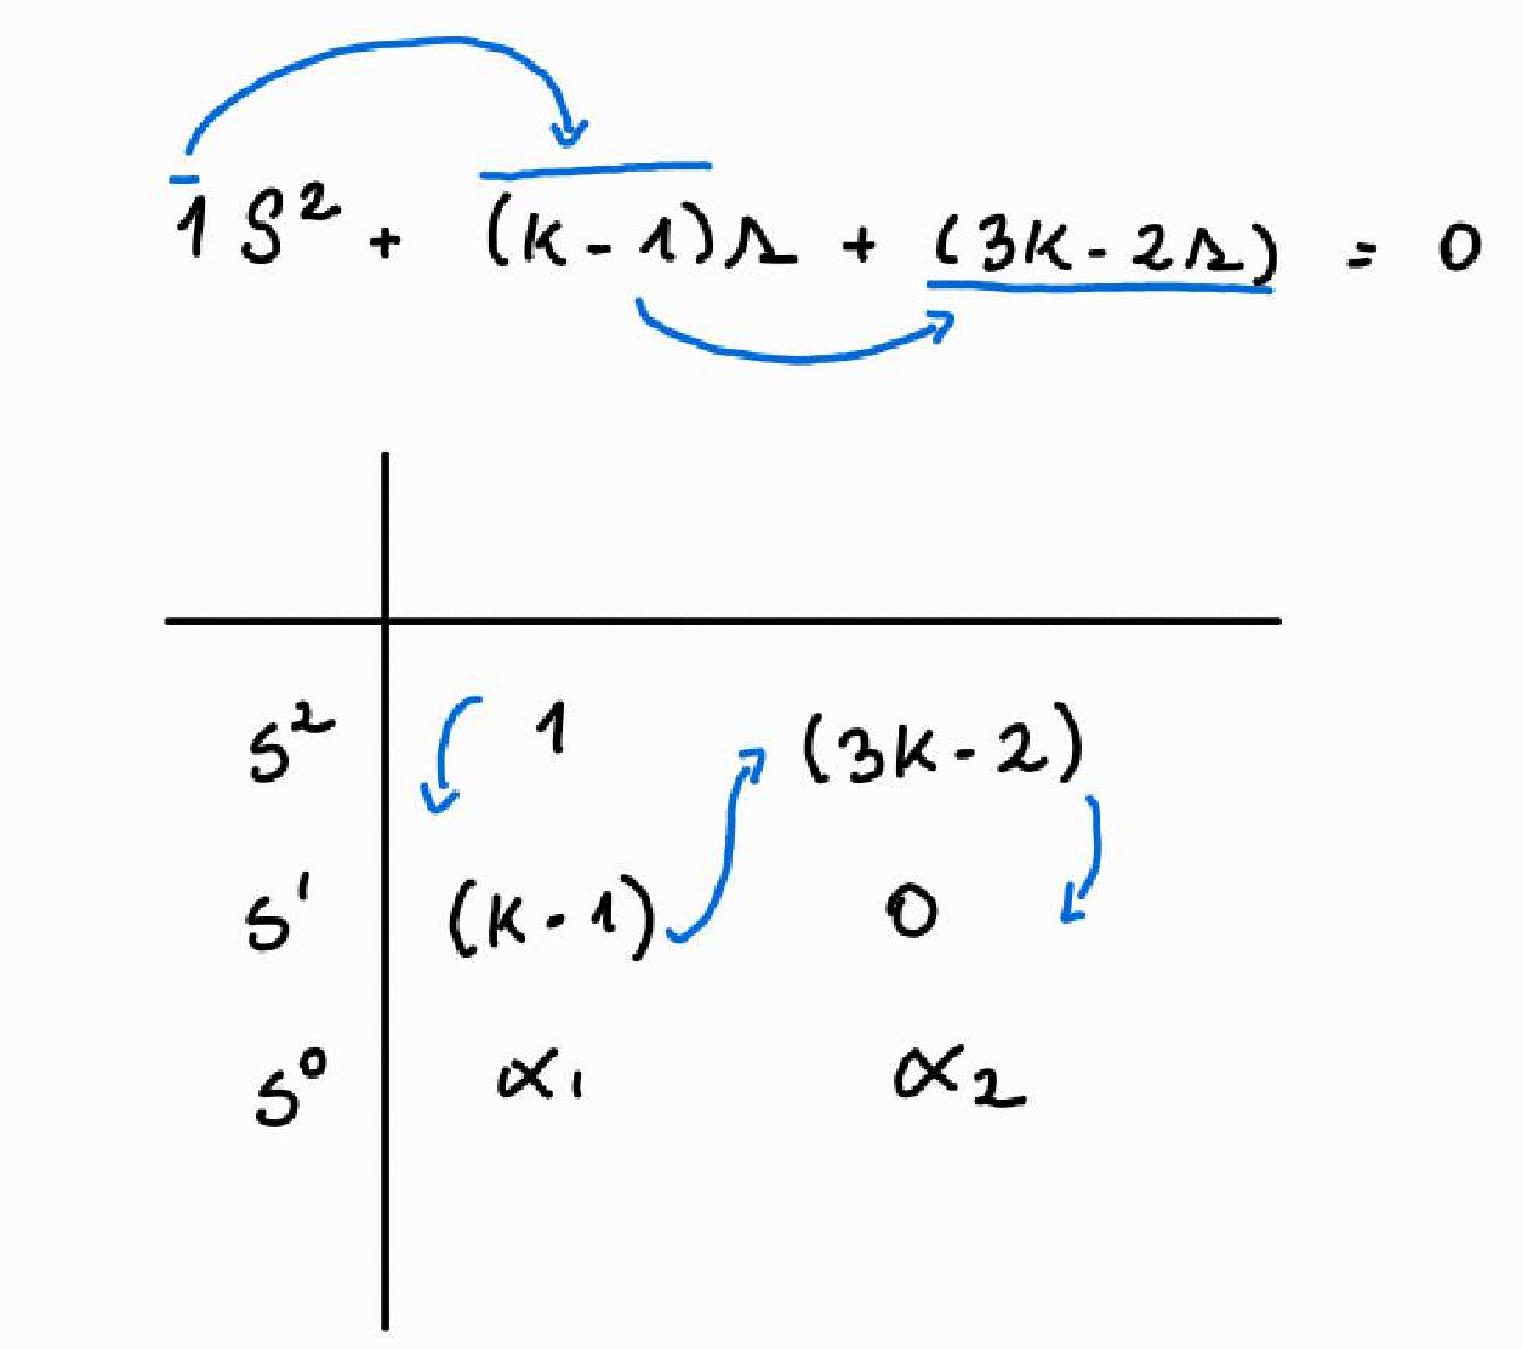
\includegraphics[width=0.5\textwidth]{Auxiliar_2_8}
    \end{center}
    \subsection*{Resolucion 3.2}
    Se busca obtener las potencias de las cargas $Z_{1}$ y $Z_{2}$, por lo que recordando que:
    
\begin{itemize}
    \item \textbf{General:}
    \begin{align}
    \frac{S_1}{S_2} &= \frac{V_1 \cdot I_1}{V_2 \cdot I_2} = \frac{N_1 \cdot N_2}{N_2 \cdot N_1} = 1 \\
    \frac{Z_1}{Z_2} &= \frac{V_1 \cdot I_2}{V_2 \cdot I_1} = \frac{N_1 \cdot N_1}{N_2 \cdot N_2} = a^2
    \end{align}

    \item \textbf{Sustractiva:}
    \begin{align}
    \frac{V_1}{V_2} &= \frac{N_1}{N_2} = a \\
    \frac{I_1}{I_2} &= \frac{N_2}{N_1} = \frac{1}{a}
    \end{align}

    \item \textbf{Aditiva:}
    \begin{align}
    \frac{V_1}{V_2} &= \frac{N_1}{N_2} = -a \\
    \frac{I_1}{I_2} &= \frac{N_2}{N_1} = -\frac{1}{a}
    \end{align}
\end{itemize}
Por lo que deberemos referencias $Z_{2}$ , por lo tanto se obtiene que:
\begin{align}
    Z'_{2} = a^{2}Z_{2} = \left(\frac{N_{1}}{N_{2}}\right)^{2}Z_{2} = \left(\frac{30}{60}\right)^{2}(20 + j) = 5 + j0.25 [\Omega]
\end{align}
\begin{center}
    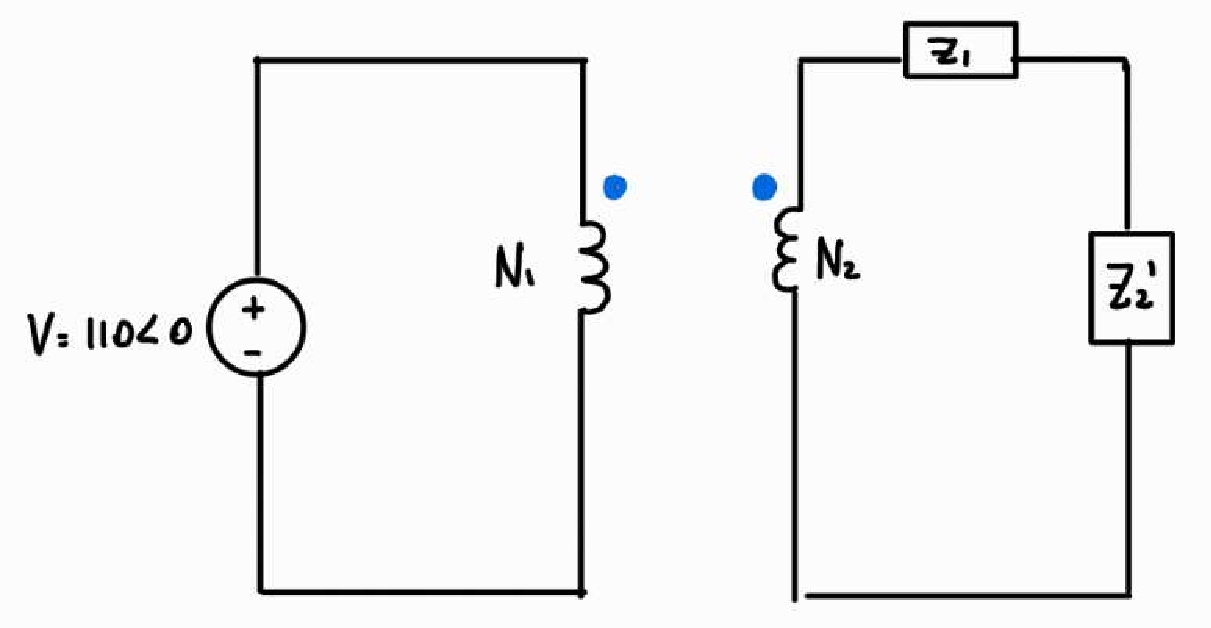
\includegraphics[width=0.4\textwidth]{Auxiliar_2_9}
\end{center}
Luego se obtiene la impedancia equivalente del circuito referenciado, la cual viene dada por:
\begin{align}
    Z_{eq}= Z_{1} + Z'_{2}= (20+j) + (5+j0.25) = 25 + j1.25 [\Omega]
\end{align}
Con esta impedancia equivalente, se referencia a el primer transformador, por lo tanto:
\begin{align}
    Z'_{eq}= a^{2}Z_{eq}= \left(\frac{N_{1}}{N_{2}}\right)^{2}Z_{eq} = \left(\frac{30}{60}\right)^{2}(25 + j1.25) = 6.25 + j0.3125 [\Omega]
\end{align}
Con lo que finalmente, es posible obtener la corriente del generador, tal que:
\begin{align}
    V &= i_{1}Z'_{eq}\\
    110\angle 0^{\circ} &= i_{1}(6.25 + j0.3125)\\
    i_{1} &= 17.6\angle -2.83^{\circ} [A]
\end{align}
Una vez obtenida esta corriente, es posible determinar la corriente de que circula originalmente por $Z_{1}$ la cual vendra dada por(\textit{Es importante notar que ocupamos las relaciones asocadas a la polaridad sustractiva}):
\begin{align}
    \frac{i_{1}}{i_{2}} &= \frac{N_{2}}{N_{1}}\\
    i_{2} & = \frac{N_{1}}{N_{2}}i_{1}\\
    i_{2} &= \frac{30}{60} \cdot 17.6\angle -2.83^{\circ} = 8.8\angle -2.83^{\circ} [A]
\end{align}
Luego para la corriente $i_{3}(t)$ que circula por $Z_{2}$ se tendra que \textit{(\textit{Es importante notar que ocupamos las relaciones asocadas a la polaridad aditiva})}:
\begin{align}
    \frac{i_{2}}{i_{3}} &= -\frac{N_{2}}{N_{1}}\\
    i_{3} &= -\frac{N_{1}}{N_{2}}i_{2}\\
    i_{3} &= -\frac{30}{60} \cdot 8.8\angle -2.83^{\circ} = -4.4\angle -2.83^{\circ} [A]
\end{align}
Luego es posible obtener S asociada a cada carga, la cual viene dada por:
\begin{align}
    S= V \cdot I^{*} = I \cdot I^{*}Z = |I|^{2}Z
\end{align}
Con lo que reemplazando para cada impedancia se tiene:
\begin{align}
    S_{Z_{1}} &= |i_{2}|^{2}Z_{1}= |8.8\angle -2.83^{\circ}|^{2}(20+j) = 386.26 + 19.3115j [VA]\\
    S_{Z_{2}} & = |i_{3}|^{2}Z_{2}= |4.4\angle -2.83^{\circ}|^{2}(20+j) = 1544.95 + 77.2477j [VA]
\end{align}
Con lo que se obtiene la potencia de ambas cargas.
\subsection*{Resolucion 3.3}
Se busca obtener la potencia de la fuente considerando dos casos para $Z_{2}$, por lo que se tiene que:
\subsubsection*{\textbf{Caso $Z_{2}=0$}}:
Considerando este caso se tendra que la impedancia sera equivalente a un corto circuito, por lo que no se tendra una impedancia equivalente, dado que tendremos solo una impedancia, asi:
\begin{align}
    Z'_{1}= a^{2}Z_{1}= \left(\frac{N_{1}}{N_{2}}\right)^{2}Z_{1} = \left(\frac{30}{60}\right)^{2}(20 + j) = 5 + j0.5 [\Omega]
\end{align}
De esta manera se tendra que la corriente del generador vendra dada por:
\begin{align}
    V &= i_{1}Z'_{1}\\
    110\angle 0^{\circ} &= i_{1}(5 + j0.5)\\
    i_{1} &= 21.9451\angle -2.86^{\circ} [A]
\end{align}
Con lo que la potencia en este caso vendra dada por:
\begin{align}
    S_{fuente} &= |i_{1}|^{2}Z_{1} = |21.9451\angle -2.86^{\circ}|^{2}(5+j0.5) = 2420 + 121j [VA]
\end{align}
\subsubsection*{\textbf{Caso $Z_{2}=\infty$}}:
Este caso resulta de manera directa , dado que se tendra que $i_{1}= i_{2}=i_{3}$ dado que es practicamente un circuito abierto y por tanto $S_{fuente} = 0 [VA]$

\end{solution}
%%%%%%%%%%%%%%%%%%%%%%%%%%%

\end{questions}
\newpage
%%%%%%%%%%%%%%%%%%%%%%%%%%%
\section{Resumen}

\begin{itemize}
    \item \textbf{Ley de Faraday} \\
    Para una espira que atraviesa un flujo magnético variable, el voltaje en [Volts] inducido en sus terminales es:
    \begin{align}
    \epsilon &= -\frac{d\phi}{dt}
    \end{align}
    
    \item \textbf{Energía Magnética} \\
    La acumulación de energía magnética en un caso sin pérdidas y con:
    \begin{itemize}
        \item 1 fuente de excitación:
        \begin{align}
        W_{fld} &= \frac{1}{2} i^2 \cdot L(x)
        \end{align}

        \item 2 fuentes de excitación:
        \begin{align}
        W_{fld} &= \frac{1}{2} i_1^2 \cdot L_{11}(x) + \frac{1}{2} i_2^2 \cdot L_{22}(x) + L_{12}(x) \cdot i_1 \cdot i_2
        \end{align}

        \item n fuentes de excitación:
        \begin{align}
        W_{fld} &= \frac{1}{2} \mathbf[{i}]^t \cdot [L] \cdot \mathbf[{i}]
        \end{align}
    \end{itemize}

    \item \textbf{Fuerza magnética} \\
    \begin{align}
    f_{fld} &= -\frac{\partial W_{fld}(\lambda,x)}{\partial x} \Bigg|_{\lambda}
    \end{align}

\end{itemize}
\end{document}